\documentclass[tikz, border=2mm]{standalone}

\usepackage{tikz}
\usetikzlibrary{calc, backgrounds}

% --- CUSTOM COLORS ---
\definecolor{garnet}{HTML}{73000A}

\begin{document}

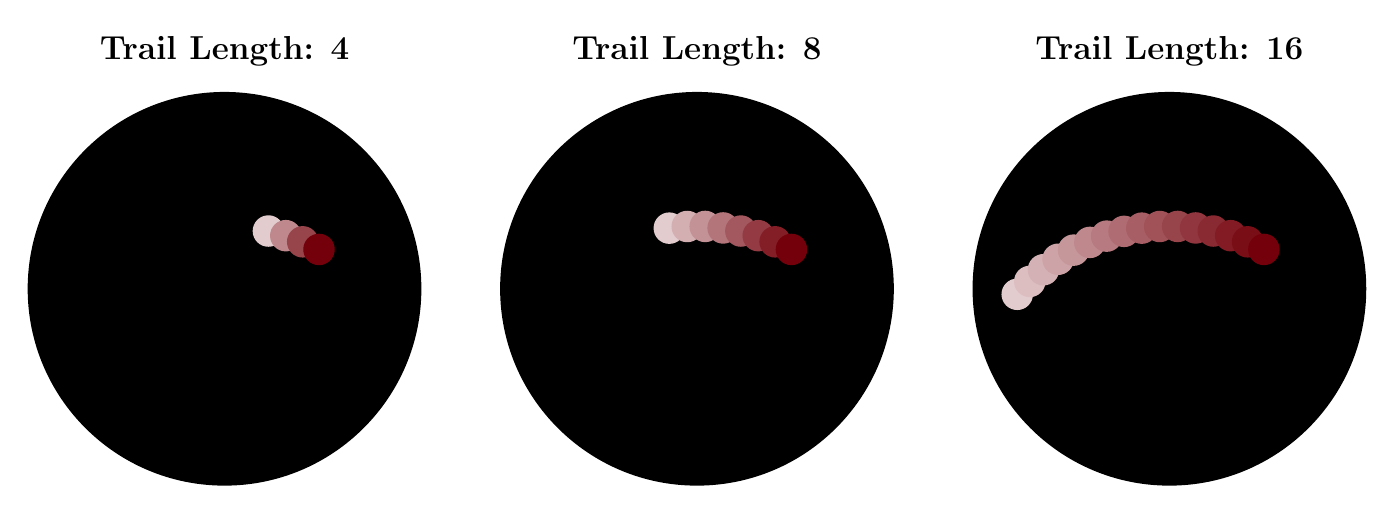
\begin{tikzpicture}

% --- MACRO: DRAW TRAIL ON CURVE ---
% #1: X Position (Center of the scope)
% #2: Number of trails (N)
\newcommand{\drawTrailCircle}[2]{
    \begin{scope}[shift={(#1,0)}]
        % Black background
        \fill[black] (0,0) circle (2.5cm);

        % Clipping region
        \begin{scope}
            \clip (0,0) circle (2.5cm);

            % --- CURVE GEOMETRY ---
            \pgfmathsetmacro{\cx}{0}
            \pgfmathsetmacro{\cy}{-1.8}
            \pgfmathsetmacro{\hx}{1.2}
            \pgfmathsetmacro{\hy}{0.5}

            \pgfmathsetmacro{\rad}{sqrt((\hx-\cx)^2 + (\hy-\cy)^2)}
            \pgfmathsetmacro{\thetaStart}{atan2(\hy-\cy, \hx-\cx)}

            \pgfmathsetmacro{\arcStepLen}{1.6/7}
            \pgfmathsetmacro{\angStep}{(\arcStepLen/\rad)*57.29578}

            \pgfmathtruncatemacro{\limit}{#2-1}

            \foreach \i in {0,...,\limit} {
                \pgfmathsetmacro{\stepsBack}{\limit-\i}
                \pgfmathsetmacro{\currentAng}{\thetaStart + \stepsBack*\angStep}

                \pgfmathsetmacro{\px}{\cx + \rad*cos(\currentAng)}
                \pgfmathsetmacro{\py}{\cy + \rad*sin(\currentAng)}

                \pgfmathsetmacro{\mix}{20 + 80*(\i/\limit)}

                \fill[garnet!\mix!white] (\px,\py) circle (0.2cm);
            }
        \end{scope}

        % Label
        \node[above, font=\bfseries\large, text=black] at (0,2.7)
            {Trail Length: #2};
    \end{scope}
}

% --- RENDER EXAMPLES ---
\drawTrailCircle{0}{4}
\drawTrailCircle{6}{8}
\drawTrailCircle{12}{16}

\end{tikzpicture}

\end{document}
